% ============================================================
% 電圧波の観測 本文
% 原本: 伝送線路_改v2.docx（である調 → です・ます調に変更）
% 担当の先生はこのファイルと figures/ だけを編集してください。
% 図のラベルは fig:voltagewave-○○ の形にしてください（他テーマとの重複防止）。
% ============================================================
\graphicspath{{contents/05_voltagewave/figures/}}

\experimenttitle{電圧波の観測}

% ============================================================
\section{目的}

電気信号伝搬の現象を観察し，理解を深めます。

% ============================================================
\section{原理}

\subsection{電気信号の伝搬}

基本的に真空中では電気信号は光速 $c$ と同等の $\SI{3e8}{m/s}$ で移動します。しかし一般的に電気信号は比誘電率をもつ絶縁体の中を移動することが多く，その伝搬速度 $v$ はその実効比誘電率 $\varepsilon_\mathrm{r}$ と光速 $c$ から
\begin{equation}
  v = \frac{c}{\sqrt{\varepsilon_\mathrm{r}}}
  \label{eq:voltagewave-velocity}
\end{equation}
と求めることができます。電気信号は速度を持つことから，電気信号が伝わる線（伝送線路）の長さによって信号の到達時間も変化します。

交流電源は電圧波高値と周波数があり，周波数 $f$（Hz）は1秒当たりの波の数であり，その逆数は周期 $T$（s）です。
\begin{equation}
  T = \frac{1}{f}
  \label{eq:voltagewave-period}
\end{equation}

% ============================================================
\section{使用器具}

\begin{equipment}
\begin{itemize}
  % TODO(原文確認): ファンクションジェネレータが「1台/部屋」と「1台/班」の2行ある
  \item ファンクションジェネレータ（1台/部屋）
  \item ファンクションジェネレータ（1台/班）
  \item ディジタルオシロスコープ \SI{50}{MHz}（1台/班）
  \item 同軸ケーブル（1本/班）
  \item BNC T字分岐コネクタ（1個/班）
  \item 終端抵抗（1個/班）
\end{itemize}
\end{equipment}

% ============================================================
\section{実験方法}

【　】の部分には，実験で得られた値を記入してください。

% ------------------------------------------------------------
\subsection{実験1：電気信号の進む速さを見てみよう！}

\begin{figure}[htbp]
  \centering
  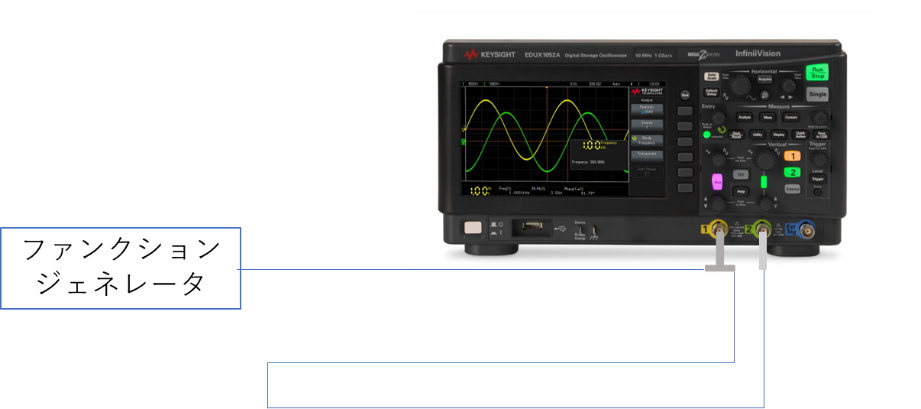
\includegraphics[width=0.75\linewidth]{voltagewave_circuit1.png}
  \caption{実験回路1}
  \label{fig:voltagewave-circuit1}
\end{figure}

\begin{procedure}[label=\textbf{(\arabic*)}, ref=(\arabic*), leftmargin=*, labelsep=0.8em]
  \item オシロスコープのch1にBNC T字分岐コネクタを，ch2に※終端抵抗を接続します。\cref{fig:voltagewave-circuit1}のようにファンクションジェネレータ出力端とオシロスコープch1のT字分岐コネクタの一端を同軸ケーブルで接続します。T字分岐コネクタのもう一端とオシロスコープのch2を長さ【　　　　】mの同軸ケーブル（RG-58A/U）で接続します。
  \item ファンクションジェネレータの電源を入れます。
  \item ファンクションジェネレータの出力を矩形波に設定して周波数を【　　　　】Hzにします。
  \item 信号の時間のずれが発生するようにオシロスコープの時間軸を【　　　　】s/Divに調整し，時間のずれを観測します。\\
    測定結果：時間のずれ【　　　　】s
  \item 観測した時間から電気信号の進む速さを算出します。\\
    計算結果：電気信号伝搬速度【　　　　】m/s
\end{procedure}

※SI接頭語（大きな数字を表すのに便利な文字）を使って適切に表しましょう（\cref{tab:voltagewave-prefix}）。

\begin{table}[htbp]
  \centering
  \caption{SI接頭語}
  \label{tab:voltagewave-prefix}
  \begin{tabular}{ccccccc}
    \toprule
    ナノ & マイクロ & ミリ & & キロ & メガ & ギガ \\
    n & μ & m & & k & M & G \\
    $10^{-9}$ & $10^{-6}$ & $10^{-3}$ & & $10^{3}$ & $10^{6}$ & $10^{9}$ \\
    \bottomrule
  \end{tabular}
\end{table}

% ------------------------------------------------------------
\subsection{実験2：定在波を見てみよう！}

\begin{figure}[htbp]
  \centering
  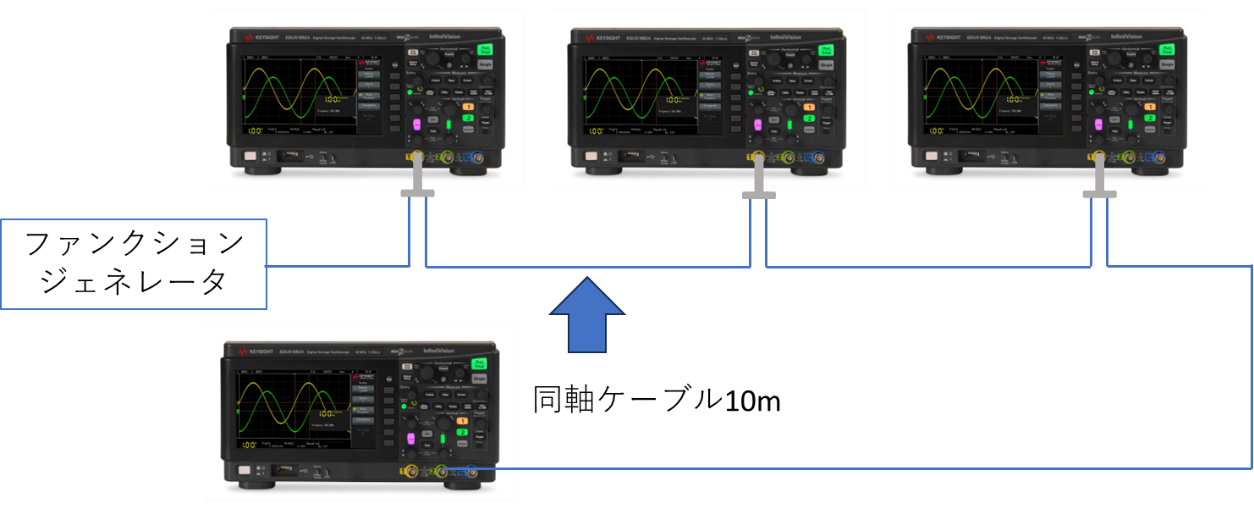
\includegraphics[width=0.9\linewidth]{voltagewave_circuit2.png}
  \caption{実験回路2}
  \label{fig:voltagewave-circuit2}
\end{figure}

\begin{procedure}[label=\textbf{(\arabic*)}, ref=(\arabic*), leftmargin=*, labelsep=0.8em]
  \item 実験1でファンクションジェネレータにつないでいたBNCケーブルを外します。
  \item オシロスコープのch2に接続していた同軸ケーブルの端子を\cref{fig:voltagewave-circuit2}のように他の班のオシロスコープの送電端（ch1）に接続し，部屋で1つのケーブルになるように接続します。
  \item 各班の同軸ケーブルの長さを表2に記録します。
  \item \label{item:voltagewave-freq} 各班の線の長さの合計【　　　　】mが波長になる周波数【　　　　】Hzを算出します。
  \item \label{item:voltagewave-table2} ファンクションジェネレータの電源を入れ，電圧値\SI{2}{V}，周波数\SI{100}{kHz}に設定し，周波数を徐々に上げます。電圧値が初めて\SI{0.5}{V}を下回った位置の同軸ケーブル長を記録します。そのときの各オシロスコープの電圧値を表2に記録します。\\
    同軸ケーブル長【　　　　】m
  % 原文は「（3）で求めた値」だが，周波数を求めるのは（4）なので参照を修正
  \item \label{item:voltagewave-table3} 周波数を\ref{item:voltagewave-freq}で求めた値まで上げた際の各班のオシロスコープの最大電圧値を表3に記録します。
\end{procedure}
